%\newtheorem{theorem}{Theorem}[chapter]
\label{algorithmic_complexity_chapter}

In this chapter, we will give a small revision of Kolmogorov complexity (K-complexity). The main objective is to explain how the library that we will use in the next chapter to measure the K-complexity works. Firstly, we will motivate the idea behind an algorithmic type complexity, suddenly the Turing machine device will be reviewed in order to be able to define this complexity, then we will discuss the former approaches to try to measure it. We will continue with some important theorems and definitions concerning the algorithmic complexity. Finally, we will describe with more detail the methodology behind the library which measures the K-complexity including some applications.

\section{The Kolmogorov Complexity}

Before we try to measure the complexity of something, we must ask: what is complexity? what makes something more complex than other things? is it possible to find a systematic way to measure complexity? but even more important, in the first place, we have to decide which kind of things we are interested to compute its complexity.  A quick search in the literature will reveal that there exist different types of complexities such as the algebraic, the computational, the linear, etc. each one with its own features and not necessarily useful for the same purposes, moreover, there is no guarantee that their measurements will coincide or be proportional when applied to the same object. There is not a universal definition of complexity, and if there were any, it would be so ambiguous, that it would not be possible to state it mathematically, and it would look almost like the definition of the Oxford dictionary which defines something which is complex simply as: "connected of many different parts. Not easy to analyze or understand; complicated or intricate" \cite{complex}. Depending on the kind of object or process we are interested, we will have to choose (or build if it does not exist) a definition of complexity that suits our interests, that allows our object or process to be measured and that fits our intuition about how the complexity of that thing should increase or decrease. Therefore, although it should be possible, for instance, to measure if one car is more complex than other, we are not interested in that specific kind of objects and complexity because it does not make any sense for our purposes. Neither we are interested, for example, in knowing if the computation of the solution of an algebraic expression is more complex than another. In this chapter, the kind of objects we want to measure its complexity are the objects that can be stored in a computer, and when we say stored, we mean that they can be represented in some way as information. So, in this kind of category, we could find an image, a text file, an audio file, etc. All these objects have in common that they are stored in a computer as sequences of bits, that is, sequences of $0's$ and $1's$. Therefore, we seek a complexity that can work with any object which can be represented as a sequence of bits. 

Now, what should we expect about the complexity of a sequence of bits? Let's consider the following sequences:
\begin{quote}
\centering
$x_{1}=01010101010101$\\
$x_{2}=00101110100101$\\
$x_{3}=00000000000000$\\
$x_{4}=11111111111111$\\
$x_{5}=0000000$
\end{quote}

The sequence $x_{1}$ is a repetition of $01$ seven times, thus it could be written just as: $x_{1}=$ "repeat $01$ seven times", making it simpler than it looks. On the other hand, the sequence $x_{2}$ has no evident repetition pattern that allows us to compress it as we did with $x_{1}$, therefore it seems $x_{2}$ is more complex than $x_{1}$. The sequences $x_{3}$ and $x_{4}$ repeat the same digit fourteen times, therefore they are highly compressible, and we should expect they are less complex than $x_{1}$. Between them, these sequences should be equally complex because they can be described by the same sentence: "repeat $\alpha$ fourteen times", where $\alpha$ is one element of the alphabet $\{ 0,1 \}$. Finally, the sequence $x_{5}$ is shorter than the former sequences and is highly compressible. Then it must be less complex than $x_{3}$. In summary:

\begin{quote}
\centering
$C(x_{5}) < C(x_{3}) = C(x_{4}) < C(x_{1}) < C(x_{2})$
\end{quote}

where $C(x_{i})$ denotes the complexity of sequence $x_{i}$. Thus, the type of complexity we are looking for must be sensitive to the next aspects:

\begin{enumerate}
	\item Between two sequences of the same length, the sequence more complex will be the less compressible sequence, or in other words the sequence with fewer regularities.
	\item This complexity must be symmetric, that is, it must be insensitive to a reflection of the alphabet elements, which means that $0101$ and $1010$ are equally complex.
	\item Between two sequences of different length containing just repetitions of a shorter sequence, the less complex of the two sequences will be the sequence with the less length.
\end{enumerate}

These observations were made for extreme cases, but our definition of complexity also must be sensitive to cases where there is no evident way to compress two sequences. For instance, for the sequences $0111011001$ and $1101000101$, there is no obvious way to compress them. Thus, we cannot say which one is more complex, however, we wish a definition of complexity which indeed can answer this question.\\ 

We also must remark two words we mentioned above: \textit{regularities} and \textit{compressible}. These two concepts are the foundation of two of the initial ways people tried to measure the complexity we are about to define. We will review these methods later in this same chapter.\\

The complexity that fulfills the previously stated needs is the \textit{algorithmic complexity} also known as \textit{Kolmogorov complexity}, \textit{K-complexity}, \textit{Kolmogorov-Chaitin complexity} or \textit{program complexity} \footnote{We will use indistinctly these names, whenever we use them, we are referring to the same definition of complexity.}. The idea behind the algorithmic complexity is to measure the complexity of an object not by the object itself but by the description that generates it. This area of study is known as algorithmic information theory. However, which kind of description should we use? and which kind of object generates the object we are talking about? A language could make a description very simple, but others could make it particularly complex. We need a universal language and a universal device which can construct objects using this universal language. To answer this question mathematicians had to wait until the advent of computer science and electronic computers, especially the ideas of Alan Turing. In fact, the idea of algorithmic complexity was not formally introduced until 1965 by the Russian mathematician Andrei N. Kolmogorov and the American mathematician Gregory J. Chaitin. An interesting historical review of the development of algorithmic complexity can be found in (\cite{kolmo_book}, pages 86-92). Hence, before we define K-complexity, we will review the Turing machine.

\subsection{The Turing Machine}
In 1936, Alan Turing proposed the machine which now is named after him to provide a simple computational model which could be used to prove formal mathematical statements \cite{hopcroft}.

It consists of an unlimited linear tape divided into cells which are coupled to a finite state machine (the machine) through a moving head which can be situated at each moment in one of the cells of the tape. This tape acts as external memory or storage where each cell or square can have a symbol from a finite alphabet set. The head performs three functions in each cycle of the finite state machine: it reads the symbol in the cell of the tape, erases the cell and writes on it a symbol (it can be the same previous symbol) according to what it has read and the rules of the program (in the machine), the machine is moved together with the head to an adjacent square (to the left or to the right) which then becomes the next cell to be scanned to continue with the next cycle (see Fig. \ref{fig:turing_machine}) \cite{marvin}.

\begin{figure}
	\centering
		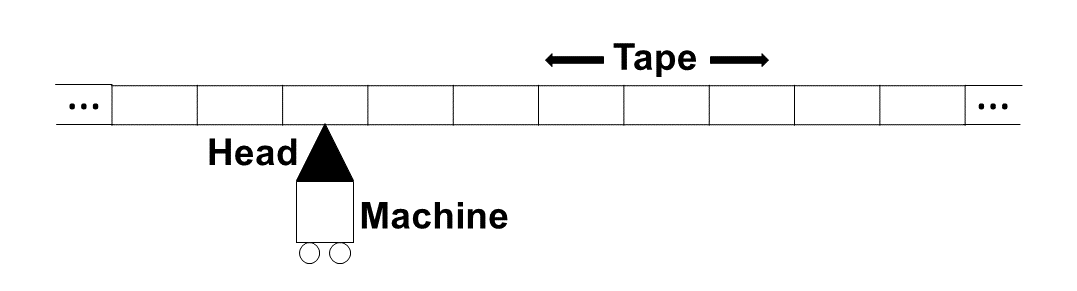
\includegraphics[width=\textwidth]{turing_machine}
	\caption{The Turing Machine.}
	\label{fig:turing_machine}
\end{figure}

Hence, we can think of a Turing machine basically as a finite state machine or finite automaton with the difference that it has unlimited auxiliary memory and the ability to reread its input and write and erase over it. This gives the Turing machine more computational power over a finite automaton but also makes it a hypothetical device\cite{judith}.
We can think in the Turing machine as the simplest computer that could exist. Nevertheless, it does not mean this theoretical machine is less powerful than any modern computer, in fact, any problem that can be solved in a Turing Machine is also solvable in a modern computer and vice versa. This is known as the Church-Turing thesis \cite{behrouz}.\\

More formally, we define a Turing machine by means of a septuple \cite{hopcroft}:

\begin{defn}
	A \textit{Turing machine} is define by means of a septuple of the form: \\
	\begin{center}
	$M=(Q, \Sigma, \Gamma, \delta,q_{0},B,F)$
	\end{center}
	where:
	\begin{itemize}
	\item $Q$ is the finite set of states of the state machine.
	\item $\Sigma$ is the finite set of input symbols.
	\item $\Gamma$ is the complete set of tape alphabet symbols ($\Sigma$ is a subset of $\Gamma$).
	\item $\delta$ is the transition function.
	\item $q_{0}$ is the initial state.
	\item $B$ is the blank space symbol.
	\item $F$ is the set of final states or accepting states which is a subset of $Q$. 
	\end{itemize}
\end{defn}

An alternative way to define a Turing machine is by describing its actions, that is by describing the behavior of the transition function $\delta$ which can be thought as the program the machine executes. This can be accomplished by means of a set of quintuples \cite{judith}:

\begin{defn}
Let $Q$ be a finite set of states and $\Gamma$ a finite set of tape symbols (the tape alphabet) including a special symbol $B$. A \textit{Turing machine} is a set of quintuples of the form $(s,i,i',s',d)$ where $ s,s'  \in Q $ ; $ i,i' \in \Gamma $ ; and $ d \in \{ R,L \} $ and no quintuples begin with the same $s$ and $i$ symbols. The symbol $s$ is the present state, $i$ is the tape symbol being scanned, $i'$ is the symbol written, $s'$ is the new state, and $d$ is the direction in which the head will be moved ($R$ is to the right and $L$ is to the left).\\
\end{defn}

The operation of a Turing Machine can be better understood through an example. Consider the Turing Machine defined by the quintuples in Table \ref{transition}. This transition table defines a parity counter, that is, a program which output will be 0 or 1 depending on whether the number of 1's in an input string of bits (the input sequence) is odd or even \cite{marvin}. The behavior of this machine for a given string is shown in Fig. \ref{fig:turing_machine}. The end of the input string is indicated to the machine with the symbol B. The machine can be in two states $q_{0}$ and $q_{1}$ which we have denoted 0 and 1 for simplicity. Likewise, we have simplified the notation for the movement of the head denoting with a 1 the movement to the right and with a 0 the movement to the left. The machine starts in the state $q_{0}$ and halts when it reaches the symbol B after it has erased the input sequence and printed the answer.

\begin{table}[h]
\centering
\begin{tabular}{ |c |c |c |c |c| }
 \hline  
 $s_{j}$ & $i_{j}$ & $i'_{j,k}$ & $s'_{j,k}$ & $d_{j,k}$ \\
 \hline \hline  
 0 & 0& 0& 0& 1 \\ 
 \hline  
 0 & 1& 0& 1& 1 \\ 
 \hline 
 0 & B& 0& H& -  \\ 
 \hline 
 1 & 0& 0& 1& 1  \\ 
 \hline 
 1 & 1& 0& 0& 1 \\
 \hline
 1 & B& 1& H& - \\
 \hline
\end{tabular}
 \caption{The transition table of a parity counter for a Turing machine. $s_{j}$ is the initial state of the machine ($0$ or $1$), $s'_{j,k}$ is the final state of the machine ($0$, $1$ or halt), $i_{j}$ is the initial symbol in the cell of the tape read by the machine ($0$, $1$ or blank), $i'_{j,k}$ is the symbol printed by the head on the cell of the tape ($0$ or $1$) and $d_{j,k}$ is the direction to which the head and the machine will be moved ($1$ means to the right, $0$ means to the left and "$-$" means there is no movement).}
 \label{transition}
\end{table}


\begin{figure}
	\centering
		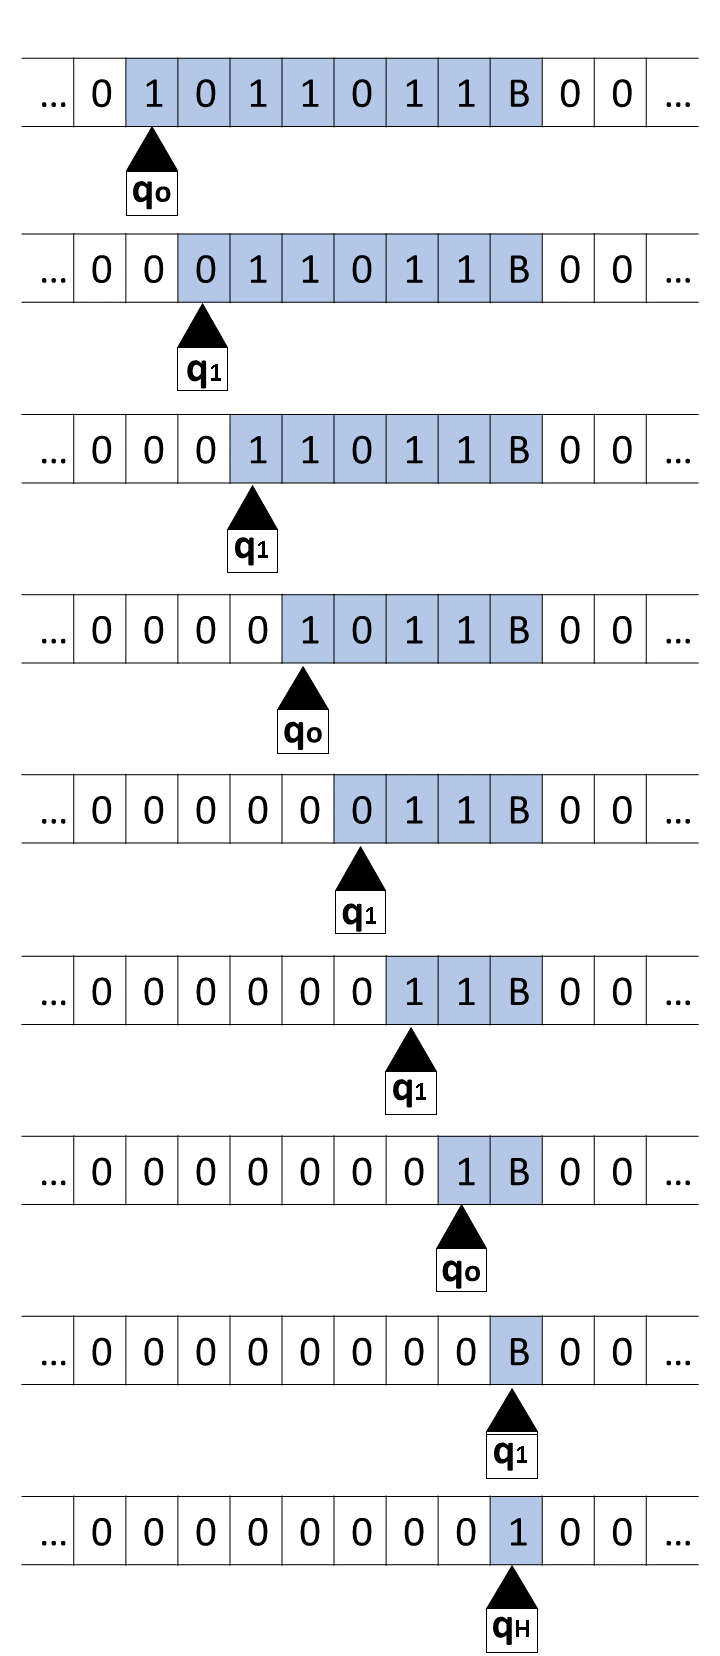
\includegraphics[scale=0.23]{parity_counter}
	\caption[A parity counter executed by a Turing machine.]{Configurations of the parity counter program shown in Table \ref{transition} in a Turing machine. The input sequence is $1011011$ which has five 1's, thus the result of the computation is $1$.}
	\label{fig:turing_machine}
\end{figure}

\subsection{The Universal Turing Machine}
We have said that a Turing Machine is the simplest theoretical example of a modern computer, although, it has a problem. Modern computers can execute multiple different programs, we do not have to buy a new computer each time we need to perform a different computation with a different set of instructions. This is not the case with a Turing machine, for instance, consider the Turing machine with the transition table given in Table \ref{transition}. This Turing machine runs a parity counter program, but what happens if now we want to run a program which computes a sum? In this case, we would have to build a brand-new Turing machine to execute this new task and we would have to do this step every time we needed to run a different program. Obviously, our current model of the Turing machine fails to mimic the ability of a modern computer to run different instructions. To overcome this problem, Turing was farther and conceived the idea of a Universal Turing Machine, a Turing machine which can simulate any other Turing machine. Or in words of Turing itself \cite{turing1936}:

\begin{quote}
It is possible to invent a single machine which can be used to compute any computable sequence. If this machine \textit{U} is supplied with a tape on the beginning of which is written the S.D\footnote{S.D stands for standard description and is the set of quintuples which define the transition table placed in a line one after the other and separated by semi-colons. Although, the convention originally proposed by Turing to order the elements in a quintuple was $(s,i,i',d,s')$ and not $(s,i,i',s',d)$ as we have agreed.} of some computing machine \textit{t}, then \textit{U} will compute the same sequence as \textit{T}.
\end{quote}

A universal Turing machine can be defined in simple words as follows \cite{utm}:

\begin{defn}
A \textit{Universal Turing Machine (UTM)} is a Turing machine which, by appropriate programming using a finite length of input tape, can act as any Turing machine whatsoever. 
\end{defn}

If we wish a more formal definition, we first ought to define a Turing-computable function as follows \cite{marvin}:

\begin{defn}
A function $f(x)$ will be said to be the Turing-computable if its values can be computed by some Turing machine $T_{f}$ whose tape is initially blank except for some standard representation of the argument x. The value of $f(x)$ is what remains on the tape when the machine stops.
\end{defn}

The standard representation used for the argument $x$ does not matter so long as we are consistent with it \cite{marvin}, so we will use a unary notation were, e.g., $x=1111$ means $4$ and $x=111$ means $3$. Thus, we can define a $UTM$ as follows \cite{marvin}:

\begin{defn}
A single, fixed $UTM$ is a machine with the property that for each and every Turing machine $T$, there is a string of symbols $d_{t}$ (which Turing called S.D) such that: if the number $x$ is written in unary notation on a blank tape, following the string $d_{t}$, and $U$ is started in $q_{0}$ on the leftmost symbol of $d_{t}$, then when the machine stops the number $f(x)$ will appear on the tape, where $f(x)$ is the number that would have been computed if the machine $T$ had been started with only $x$ on its tape.
\end{defn}

The former statements help to give a more formal definition of a universal Turing machine; however, it is possible to give an even more general definition (see \cite{taylor}, page 140-144). An example of a Universal Turing Machine can be seen in Fig \ref{fig:UTM}. An implementation of a UTM can be found in (\cite{marvin}, page 143-144).

\begin{figure}
	\centering
		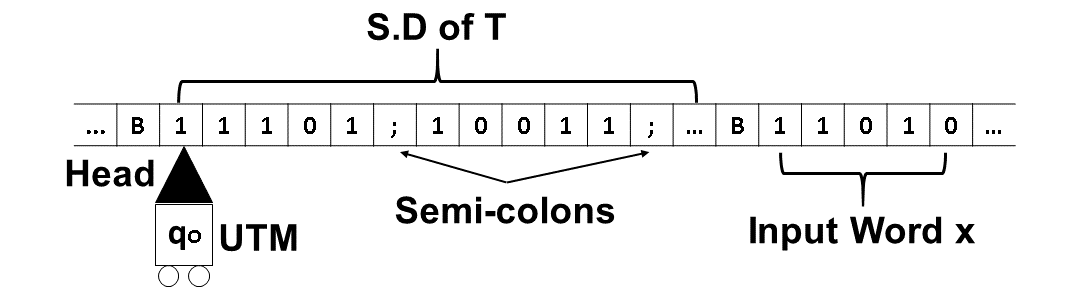
\includegraphics[width=\textwidth]{UTM}
	\caption[A universal Turing Machine.]{A universal Turing Machine $U$. The head of $U$ starts in the state $q_{0}$ and begins scanning the leftmost symbol of the standard description (S.D) of the Turing machine $T$ which $U$ simulates. The S.D of $T$ is created by putting the quintuples of $T$ one after each other and separating them by semi-colons. After the S.D of $T$, the input word $x$ is placed in unary notation. The computation of $U$ will give $f(x)$, the same result that the computation of $T$ would have given if it had started only with $x$ on its tape.}
	\label{fig:UTM}
\end{figure}

\subsection{The Halting Problem}
\label{halting_problem}
When we use a Turing machine and a determined tape to perform a computation, in some situations the process to get a result may take just a few steps but in others, it could require much more time. In fact, the execution could take a lot of time that it becomes impractical, or even it could never halt. Thus, for practical reasons, we would like to have a way to know the time it will take the machine to halt or just confirm before we start the computation if the execution will ever halt. This is known as the halting problem and can be formulated as \cite{judith}:

\begin{defn}
The \textit{halting problem} asks, does an algorithm exist to decide, given any Turing machine $T$ and string $x$, whether $T$ begun on a tape containing $x$ will eventually halt?
\end{defn}

Unfortunately, the following theorem which can be proved gives an answer to the halting problem \cite{judith} \cite{marvin}:

\begin{theorem}
The halting problem is unsolvable.
\end{theorem}

Although the halting problem for a general Turing machine is unsolvable, this problem is solvable for machines with less than four states, furthermore, the four-state problem is open, and the five-state problem is almost certainly unsolvable \cite{halting}.

A special case of the halting problem is the blank-tape halting problem \cite{marvin}:

\begin{defn}
Is it possible to build a machine which will decide, for each machine $T$, does $T$ halt if started on a blank tape?
\end{defn}

Evidently, this special case is also unsolvable for a general Turing machine, however, this also means that the special cases for machines with just a few states do have a solution as stated for the general halting problem. Indeed, the Busy Beaver functions solve the problem, but we will return to this point later when we discuss the methodology which has been used to measure the Kolmogorov complexity.

\subsection{The Formal Definition of K-Complexity}
Prior to being able to formally define K-complexity, we ought to build a theoretical framework to make immediately easy to understand its definition. This is because this definition was the result of a process which took several years to be completed and many concepts had to be introduced and clarify before we could reach a satisfactory universal definition of complexity, see (\cite{kolmo_book} , pages 86-92 and pages 47-49) and footnote 3 in (\cite{kolmo_book2}, pages 122-123).\\

We will work with sequences or strings \footnote{We will use indistinctly these names as synonyms.} of elements which belong to the nonempty set $B=\{0,1\}$. The set of all finite strings over $B$ is denoted $B^{*}$, where $B^{*}=\{ \emptyset,0,1,00,01,10,11,000,001,... \} $ and $\emptyset$ is the empty sequence \cite{kolmo_book}. There is a widely used, though not one-to-one\footnote{It is not one-to-one because for example both $"100"$ and $"0101"$ map to the same number $5$.} correspondence of $B^{*}$ onto the natural numbers such that $"100"$ maps to $4$ and $101$ maps to $5$. It is known as counting in base $2$ or binary representation. These sequences are represented such that \cite{kolmo_book}:\\

\begin{defn}
If $x$ is a string of $n$ $0's$ and $1's$, then $x_{i}$ denotes the $i$th bit (binary digit) of $x$ for all $i$, $1 \leq i \leq n$, and $x_{i:j}$ denotes the $(j-i+1)$-bit segment $x_{i} x_{i+1} ...x_{j}$.
\end{defn}

For example, for $x=1101$, we have $x_{1}=x_{2}=x_{4}=1$ and $x_{3}=0$. We will consider binary strings of different lengths \cite{kolmo_book}:

\begin{defn}
\label{length}
The \textit{length} of a binary string $s$ is the number of bits it contains and is denoted by $l(s)$ or $|s|$.
\end{defn}

We can consider decoding functions which are defined next \cite{kolmo_book}:
\begin{defn}
If $D$ is any function $D: \{0,1\}^{*} \rightarrow N$, then if we consider the domain of $D$ as the set of \textit{code words}, and the range of $D$ as the set of \textit{source words}, $D(y)=x$ is interpreted as "$y$ is a code word for the source word $x$, and $D$ is the  \textit{decoding function}. The set of all code words for source word $x$ is the set $D^{-1} (x)=\{y:D(y)=x\}$ and $E=D^{-1}$ is the encoding relation (or encoding function if $D^{-1}$ happens to be a function).
\end{defn}

Following it is necessary to introduce the concept of prefix-free codes \cite{kolmo_book}:

\begin{defn}
Let $x,y \in \{0,1\}^{*}$. Then we call $x$ a \textit{prefix} of $y$ if there is a $z$ such that $y=xz$.
\end{defn}

For instance, the string $10$ is a prefix of $1011010$ where $x=10$, $y=1011010$ and $z=11010$.  In addition, we define a prefix-free set as \cite{kolmo_book}:

\begin{defn}
A set $a \subseteq \{0,1\}^{*}$ is \textit{prefix-free}, if no element in $A$ is the prefix of another element in $A$.
\end{defn}

Furthermore, we have that \cite{kolmo_book}:
\begin{defn}
A function $D: \{0,1\}^{*} \rightarrow N$ defines a \textit{prefix-code} if its domain is prefix-free.
\end{defn}

\begin{defn}
A code is a \textit{prefix-code} or \textit{instantaneous} if the set of code words is prefix-free (no code word is a prefix of another code word).
\end{defn}

With the former definitions in mind we can define a prefix-free Turing machine \cite{decomposition}:
\begin{defn}
\label{prefix-free}
A Turing Machine is said to be \textit{prefix-free} if the group of its valid programs forms a prefix-free set (no element is a prefix of any other).
\end{defn}

Or in other words:
\begin{quote}
A \textit{prefix-free function} is one whose domain is prefix-free. Similarly, a \textit{prefix-free Turing machine} is one whose domain is prefix-free. It is usual to consider such a machine as being \textit{self-delimiting}, which means that it has a one-way read head that halts when the machine accepts the string described by the bits read so far. The point is that such a machine is forced to accept strings without knowing whether there are any more bits written on the input tape. This is a purely technical device that forces the machine to have a prefix-free domain, but it also highlights how the use of prefix-free machines circumvents the use of length to gain more information (\cite{kolmo_book2}, page 122).
\end{quote}
Now we have the framework necessary to present the formal definition of the K-complexity \cite{decomposition}:

\begin{defn}
\label{k_complexity_formal_def}
The \textbf{\textit{algorithmic complexity}} $K(S)$ of a string $S$ is the length\footnote{See Definition \ref{length}.} of the shortest program $p$ that outputs the string $S$, when running on a universal (prefix-free) Turing machine U. That is:

\begin{equation}
  K(S)=min \{ |p| : U(p)=S \}
\end{equation}

where $|p|$ is the length of the program $p$ and $K(S)= \infty $ if there are no such $p$.
\end{defn}

Unfortunately, the cost of being a universal definition of complexity \footnote{This measure of complexity is said to be universal because it has been proved to be robust since several independent definitions converge to it, thus making it reliable \cite{kolmo_calculating}.} is that it is incomputable, i.e., there is no such function $K$ which accepts a sequence $S$ and returns the length of the shortest program which produces $S$. Nonetheless, the upper bound of Kolmogorov complexity is computable, so it is called upper semi-computable or lower semi-computable \footnote{Upper in the sense that the upper bound can be found and lower in the sense that it is an approximation.} \cite{decomposition}. In the next section, the former approaches to try to approximate the K-complexity will be reviewed.

\section{Lossless Compression and Entropy as Approximations to K-Complexity}
The concepts of algorithmic information theory were born as problems in the frontiers of probability theory and information theory. In fact, the original purpose of the definition of algorithmic complexity was to define randomness: "If the shortest program $p$ producing $s$ is larger than $|s|$, the length of $s$, then $s$ is considered random" \cite{kolmo_calculating}. Therefore, its origins give a clue in how we can approximate K-complexity by using compression methods and entropy measurements which can detect regularities in data sequences. We will begin discussing lossless compression as an approximation to K-complexity to continue with entropy as another approximation.

\subsection{The Lossless Compression}
Theoretically, a compression function is defined as \cite{kolmo_compression}:

\begin{defn}
A \textit{compression function} is a computable function $q$ such that $U(q(x))=x$, for all strings $x$ for some fixed universal Turing machine. The trivial compression function $q(x)$ simply outputs the program \textit{"print x"}.
\end{defn}

To be called lossless compression it has to exist an inverse function which fully recovers the original data $x$ from $q(x)$, i.e., the function $U$, in a process called decompression \footnote{If the information cannot be fully recovered it is called lossy compression (see \cite{info_theory}, page 119). We are only interested in lossless compression so whenever we say compression, we are referring to it.}.
Thus, we can see a compression algorithm as a function which maps an input string $x$ onto other string $y$ which is written using the same alphabet units of $x$. \footnote{If the resulting string $y$ is written using the same alphabet units, the process is called data compression otherwise it is called data encoding \cite{decomposition}}. The goal of a compression method is that the length of the resulting string $y$ plus the length of the instructions needed to reconstruct $x$ (in our definition the instructions of the Turing machine) must be less than the original length of $x$. 
Among the most famous lossless compression algorithms, we can cite the Huffman Coding which creates a compressed code by means of an extended binary tree which takes into account the relative apparition frequency of sequence elements of a string (we briefly mentioned it in Section \ref{trees}) (see \cite{info_theory}, pages 131-133). Other famous methods are the Lempel-Ziv algorithms (LZ77 and LZ78) which are dictionary-based methods in which a dictionary of phrases is used to replace elements indicated by pointers in the string. Nowadays, variations of Lempel-Ziv algorithms are widely used to get compressed files in well-known extensions such as LHarc, PKZIP, GNU ZIP (GZIP), Info-ZIP, Portable Network Graphics (PNG), PDF, etc (see \cite{info_theory}, page 229). One of the most important derivations is the DEFLATE algorithm which uses at the same time a combination of the LZ77 and Huffman methods \cite{deflate}.\\

Nonetheless, it does not matter which compression algorithm we choose, there will always be at least one file which will not be compressed to a smaller size if we try to do it \cite{decomposition}:

\begin{proof}
Strings of data of length $N$ or shorter are clearly a strict superset of the sequences of length $N-1$ or shorter. It follows therefore that there are more data strings of length $N$ or shorter than there are data strings of length $N-1$ or shorter. And it follows from the \textit{pigeonhole principle} that it is not possible to map every sequence of length $N$ or shorter to a unique sequence of length $N-1$ or shorter. Therefore, there is no single algorithm that reduces the size of all data.
\end{proof}

Then it is necessary to have a way to quantify the goodness of compression. One way is with the compression ratio (\cite{info_theory}, page 119):

\begin{defn}

\begin{equation}
  compression ratio= \frac{|x|}{|q(x)|}
\end{equation}

\end{defn}

If the compression ratio is greater than one it means that the compression algorithm worked otherwise it was not helpful. However, we must have in mind that this ratio does not consider how fast the algorithm works or how many information was preserved, and furthermore, it says nothing about the length of the instructions necessary to recover $x$. Nevertheless, in lossless compression methods, all the information is always preserved, and the length of the instructions are usually negligible (\cite{info_theory}, page 119). \\

Initially, the lossless compression methods were mainly used as a measure of Kolmogorov complexity because compression is enough to test for non-algorithmic randomness (though the converse is not true) and provides an upper bound to K-complexity \cite{decomposition}. Therefore, the size of a compressed file is an approximate measurement of K-complexity and the most we can compress a file the less complex it is \cite{universos}. This compressed file can be thought as a program whose size is approximately the size of the shortest program $p$ that outputs the string $s$ when is decompressed \cite{faibles_complexites}. With this approximation, it was possible to give practical applications to K-complexity in text classification, music \cite{faibles_complexites}, bioinformatics (genetic sequences) \cite{bio_compression1} \cite{bio_compression2} and clustering \cite{clustering}. An elegant experiment demonstrating compression capabilities carry out by ants in nature is briefly reviewed in (\cite{kolmo_book}, page 583).\\

The main problem with compression methods is that as was said, there is no single algorithm which can compress every string to a shorter size. This problem is more serious with short sequences since it is common that the result of applying a compression method to a short sequence will be a larger sequence due to certain data structures, headers, etc \cite{universos}. Besides, there is also a theoretical problem with this approach to short sequences: there is no way to further compress a single bit, which would mean that a single bit has maximal complexity. This result does not make any sense according to the intuition aspects we talk about at the beginning of the chapter and restricts the use of compression algorithms as an approximation of Algorithmic Complexity only for large sequences (larger than hundreds of bits)\cite{faibles_complexites}. The main problem is that compression methods, like the LZ algorithms, work looking for repeated sequences \footnote{There also exist probabilistic based compression algorithms, though the user usually does not have a way to update or infer a good statistical model of the source thus making necessary to use methods like the LZ (see \cite{decomposition} and \cite{info_theory} pages 193-195).}, i.e., statistical regularities (redundancy) and not for algorithmic ones which make this approach no better than entropy-based estimations which we continue discussing in the following section.

\subsection{The Shannon Entropy}
Now we devote to briefly review the concept of entropy in information science. The branch of mathematics called information theory had its birth with a paper published by the American mathematician Claude Shannon in 1948: "A mathematical theory of communication"\cite{shannon}. Shannon was concerned with the problem of transmitting a message under the assumption that the ensemble of possible messages is known for both the sender and receiver no matter which meaning it could have (\cite{kolmo_book}, page 65). Therefore, its measure of information does not take into account the content of the message but the action itself of choosing a message to communicate from an ensemble is what it cares about \footnote{Opposite to Kolmogorov approach where we do measure the information contained in an object (\cite{kolmo_book}, page 65)}. If the reader has taken a course in statistical physics he should have started to relate this approach with the notion of an ensemble of particles and the probability of finding a given state which in one way or another finishes hooked to the definition of entropy also known as Gibbs or Boltzmann entropy in this context. In fact, in a particular case, the Gibbs entropy is proportional to Shannon's entropy (\cite{kolmo_book}, page 565) \footnote{The study of entropy has its roots in the sunrise of thermodynamics and its second law in the nineteenth century with the work of Sadi Carnot, Clausius, et al. (See \cite{termo}, chapters: 6,7, and 8)}. Besides the thermodynamics and statistical versions of entropy, we have a related definition of entropy in information science. Although the most common definition in computer science is that given by Shannon, there exist alternative definitions of entropy as the Kolmogorov-Sinai and the Rényi entropies which measure the amount of information needed to transmit the description of an object and rely on the assumption that the uncertainty measured by entropy is a non-decreasing function of the amount of information \cite{kolmo_graph}. Thus, all of them exhibit the same behavior: Systems with low entropy are those with a little amount of information available and we can consider them simple \cite{kolmo_graph}. Several other types of entropy definitions have been developed for specialized and punctual applications \cite{kolmo_graph}. Despite this zoo of possible definitions, we will only work with the original statement of Shannon entropy which is defined as \cite{info_theory}.

\begin{defn}
Let $s$ be an event or phenomenon with a priory probability $P(s)$ of occurrence. We define the \textit{amount of information disclosed or given off by the occurrence of and event s} as:

\begin{equation}
  I(s)=log(\dfrac{1}{P(s)})=-\log_{b}(P(s))
\end{equation}

If $P(s)=0$ then $I(s)= \infty $.
\end{defn}

\begin{defn}
Let $s_{1},...s_{n}$ an ensemble of possible events which are pairwise mutually exclusive with $\sum_{i=1}^{n} P(s_{i}) = 1$, then the average information of an event in the list ensemble or the \textit{Shannon entropy} is:

\begin{equation}
  H(s_{1},...s_{n})=\sum_{i=1}^{n} P(s_{i}) I(s_{i}) = -\sum_{i=1}^{n} P(s_{i}) \log_{b} P(s_{i})
\end{equation}

\end{defn}

Although the base of the logarithm usually is taken to be $e$ by convention, sometimes this election depends on the number of alphabet elements we are working with, e.g., when working with binary sequences we can take the base of the logarithm to be $2$. This election is not a big problem as the only effect it has is to multiply by a constant the result. If we consider the ensemble of possible events $s_{1},...s_{n}$ as a discrete random variable $S$ with given probabilities $P(S=s_{i})=p_{i}$ we write the \textbf{Shannon entropy} as:

\begin{equation}
\label{entropy}
  H(S)= -\sum_{i=1}^{n} P(s_{i}) \log_{2} P(s_{i})
\end{equation}

If $P(s_{i})=0$ we take $\log_{2}$ to be $0$. This definition is generalized in the case of a continuous random variable \cite{kolmo_graph}:

\begin{defn}
Given a variable $S$ with $n$ possible discrete outcomes such that in the limit $n\to\infty$ the density of $S$ approaches the invariant measure $m(s)$, the \textit{continuous entropy} is given by:

\begin{equation}
  \lim_{n\to\infty} H(S)=- \int P(s) \frac{P(s)}{m(s)}dx \\
\end{equation}

\end{defn}

Shannon conceived its definition of entropy as a measure of the information transmitted over a stochastic channel when the alphabet elements are known and established hard limits to maximum lossless compression rates \cite{decomposition}.\\

Now, we will see how we can use Eq. \ref{entropy} through an example. Consider tossing a coin with equal probabilities of coming up heads or tails, i.e., $P(h)=P(t)=0.5$. In this case, we have only two possible values or results when tossing the coin hence, when applying the entropy definition, we get:

\begin{flalign*}
  H(toss)=-P(h)\log_{2}P(h)-P(t)\log_{2}P(t)\\
  =-0.5\log_{2}(0.5)-0.5\log_{2}(0.5)\\
  =-\log_{2}(0.5)=1
\end{flalign*}

Therefore, to send a message with the result of tossing a coin we would need to send one bit of information. In case we need to send the result of tossing the coin 10 times we would need to send 10 bits of information. This is the event with maximal entropy as the equal probabilities imply maximal uncertainty about the result of tossing a coin. However, if we now consider a loaded coin with unequal probabilities of getting heads or tails such that $P(h)=0.2$ and $P(t)=0.8$ we would get: 

\begin{flalign*}
  H(toss)=-P(h)\log_{2}P(h)-P(t)\log_{2}P(t)\\
         =-0.2\log_{2}(0.2)-0.8\log_{2}(0.8)\approx 0.721<1
\end{flalign*}

This means to transmit the result of tossing a loaded coin we need less than one full bit. In case we need to send the result of tossing this loaded coin 10 times we would need to send in the optimal case with the optimal encoder around only 7 bits of information\footnote{Of course we can send 10 bits of information with the result of every event, however, less entropy means that it is possible to encode the result of tossing the loaded coin 10 times in a way we need less than 10 bits. In this case, with the most optimal encode we would need around 7 bits.}. The unequal probabilities have reduced the uncertainty of tossing the coin which means the event of getting a result contains less information than the original coin with equal probabilities, i.e., the event of tossing a loaded coin has less entropy. 

In the experiment of tossing a coin we only have two possible results, but we can have events with more results. For instance, consider an event $X$ where the result can take five different values $\{a,b,c,d,e\}$ with probabilities: $\{P(a)=0.2,P(b)=0.1,P(c)=0.5,P(d)=0.1,P(e)=0.1\}$. In this case the entropy is:

\begin{align*}
  H(X)=-P(a)\log_{5}P(a)-P(b)\log_{5}P(b)-P(c)\log_{5}P(c)
  \\-P(d)\log_{5}P(d)-P(e)\log_{5}P(e)\\
      =-0.2\log_{5}(0.2)-0.1\log_{5}(0.1)-0.5\log_{5}(0.5)
      \\-0.1\log_{5}(0.1)-0.1\log_{5}(0.1)\\
      =-0.2\log_{5}(0.2)-0.5\log_{5}(0.5)-0.3\log_{5}(0.1)\\
      \approx 1.9>1
\end{align*}

This means we need almost 2 bits of information to transmit the result of an event, and in case we need to send the result of 10 events we would need around 20 bits in the most optimal case where we use the optimal encoder.\\

Nevertheless, it must be remarked, that in the last examples we are not talking about sending a set of results, i.e., we are not assigning these entropies to a sequence but rather we are calculating the entropy of a stochastic source.\\

In the case of a sequence, e.g., the sequence $1110101$. First, we count the number of occurrences of the two possible outcomes. With this information can build the random variable which generated the sequence, in our case we get $S=\{s_{0}=0.285,s_{1}=0.715 \}$. Therefore, applying Eq. \ref{entropy} we get $H(S)=0.863$.\\

However, what happens if we wish to know the amount of information needed to send the result of tossing two coins at the same time? i.e., the experiment of getting a result given that we got another result formerly. We could perform a tossing and send the result and then perform another tossing and again send the result. However, in some cases is a better and more efficient idea to first perform the experiments and then transmit the results. For such cases we define the joint entropy (\cite{kolmo_book}, pages 68-69):

\begin{defn}
Let the \textit{joint probability} $P(X,Y)$ of\footnote{Some authors use the notation $P(X \cap Y)$ for the joint probability of events $X$ and $Y$ and $H(X \cap Y)$ for the joint entropy, this is in conformity with the notation for the intersection of two event sets $X \cap Y$ however, we will use the simpler notation $P(X,Y)$ and $H(X,Y)$} the random variables \textit{X} and \textit{Y} be defined by: "$P(a,b)$ is the probability of the joint occurrence of event $X=a$ and event $Y=b$, i.e., the probability of event $Y=b$ occurring at the same time that event $X=a$ occurs. Hence, the \textit{joint entropy} is given by:

\begin{equation}
\label{joint_entropy}
  H(X,Y)=-\sum_{X} \sum_{Y} P(X,Y) \log_{b} P(X,Y)\\
\end{equation}

\end{defn}

Now we can know the entropy of tossing two coins at the same time. Nonetheless, what if now we wish to toss 1000 coins at the same time? or if we want to know the entropy associated with a long sequence of events as $101010...10$. This sequence is generated by repetition of the bits $10$ and has the same number of $0's$ and $1's$, thus given these number of occurrences we have a random variable such that $S=\{s_{0}=0.5,s_{1}=0.5 \}$. If we use Eq. \ref{entropy}, we will get that this sequence (or more precisely the source that generated it) has maximal entropy (this is just the example of a fair coin which discussed before), even though this sequence was generated in a very simple way. This result represents a problem if we want to use Shannon entropy to measure Kolmogorov complexity. According to Kolmogorov's ideas this sequence has low complexity. This problem arises because with the Eq. \ref{entropy} we can only study the smallest granularity (1 bit) or 1-symbol block \footnote{We are assuming a uniform probability distribution for the $0's$ and $1's$ and for sequences of the same finite length.} of the sequence. On the other hand, if we use Eq. \ref{joint_entropy}, we could study the entropy associated with blocks of length two. This could give a result that better captures the complexity of this sequence, but moreover, there should exist an optimal block length in which the entropy we get is minimal which would be in accordance with Kolmogorov complexity. Hence, for our purposes, it is necessary to generalize Eq. \ref{joint_entropy} to consider blocks of length $n$ \cite{entropy_wolfram}:

\begin{defn}
The \textit{joint entropy} of variables $X_{1},...,X_{n}$ is given by:

\begin{equation}
\label{joint_entropy_general}
  H(X_{1},...,X_{n})=-\sum_{X_{1}} \cdots \sum_{X_{n}} P(x_{1},...,x_{n}) \log_{b} [P(X_{1},...,X_{n})]
\end{equation}

where $P(x_{1},...,x_{n})$ is the probability of obtaining the combination of $n$ symbols corresponding to a given block.\\
\end{defn}

Finally, for infinite or very long sequences originated from a stationary source, we define the entropy rate of a sequence $S$ as \cite{decomposition}:

\begin{defn}

\begin{equation}
  \lim_{n\to\infty} \frac{1}{n} \sum_{|s'|=n} H_{n}(s')
\end{equation}

where $|s'|=n$ indicates we are considering all the generated strings of length $n$.\\
\end{defn}

As was said before, entropy gives a clue in how much a finite sequence can be compressed, giving it a useful application for data compression. In fact, we can consider entropy as a measure of the amount of information that a finite sequence has \cite{decomposition}. Besides, it has been used as an approximation to Kolmogorov complexity, even though, it is an imperfect approximation for the simple reason that it is a computable function \cite{decomposition}. The best performance of Shannon entropy as an approximation of Kolmogorov complexity is gotten when a given sequence is partitioned in blocks of increasing size up to half the total length of the string. Then the entropy of the sequence is calculated for each one of these block lengths by means of Eq. \ref{joint_entropy_general}. The best measure will be that with the block length that minimizes the entropy of the sequence, meaning that that partitioning better captures the periodic statistical regularities of the sequence \cite{decomposition}.\\

The entropy is a bad approximation of Kolmogorov complexity due to the fact it only considers the frequency of occurrence of the events $0$ and $1$, i.e., it does not capture algorithmic features of the generative process \cite{faibles_complexites}. Moreover, the value of Shannon entropy can be different for different invariant representations of the same object. This is the case of graphs since it has been shown empirically that the value of the entropy is strongly influenced by the representation used to describe the graph. Furthermore, entropy cannot consider more than one feature at the same time. All this gives as result high complexities to some graphs which should be classified as not complex (for a complete discussion of why entropy is a bad measure of graph complexity see \cite{kolmo_graph} section 2.2).


\section{Towards a Better Measurement of K-Complexity}
The former discussion of lossless compression and Shannon entropy methods gives us the conclusion that we must search a better way to approximate Kolmogorov complexity. Due to the enormous amount of issues they have, both methods fail to provide a robust estimation to K-complexity.\\ 

An implementation which approximates Algorithmic Complexity has already been published, but before we try to understand how it works, we will present some definitions and theorems which will pave the road.


\subsection{The Invariance Theorem}
In Definition \ref{k_complexity_formal_def}, we saw how Kolmogorov complexity is defined by means of a UTM, however, to which UTM is this definition referring? If we expect this definition to be robust enough to be considered a universal measure of complexity, this definition must be independent of the UTM chosen to measure K-complexity. This behavior is guaranteed by the invariance theorem which states that we can guarantee the convergence of the K-Complexity no matter what universal Turing machine we are using, this is because, in the end, every lossless description can be translated to another just by using a program of fixed length, which means the K-complexity will be equal up to a constant which we hope will be negligible for long sequences, that is (\cite{decomposition}, also see pages 103-104 of \cite{kolmo_book}):

%One of the main differences between Kolmogorov Complexity and other measures like entropy ones is that the K-complexity of an object is invariant to different lossless descriptions. In other words, we can guarantee the convergence of the K-Complexity no matter what universal Turing machine we are using, this is because, in the end, every lossless description can be translated to another just by using a program of fixed length, which means the K-complexity will be equal up to a constant which we hope will be negligible for long sequences. This behavior is guaranteed by the invariance theorem which states that (\cite{decomposition}, also see pages 103-104 of \cite{kolmo_book}):

\begin{theorem}[Invariance Rate]
If $U_{1}$ and $U_{2}$ are two \textit{UTMs} and $K_{U_{1}}$ and $K_{U_{2}}$ the algorithmic complexity of $S$ for $U_{1}$ and $U_{2}$, there exists a constant $C_{U_{1},U_{2}}$ such that:

\begin{equation}
  |K_{U_{1}}(S)-K_{U_{2}}(S)|<C_{U_{1},U_{2}}
\end{equation}

where $C_{U_{1},U_{2}}$ is independent of $S$ and can be considered to be the length (in bits) of a translating function between universal Turing machines $U_{1}$ and $U_{2}$, or as a compiler between computer programming languages $U_{1}$ and $U_{2}$.
\end{theorem}

The size of the constant $C_{U_{1},U_{2}}$ is unknown an can be arbitrarily large, although we can expect that for long sequences, the approximation with a machine $U_{a}$ will converge to the true value \cite{decomposition}, i.e., $K_{U_{a}}(S) \sim K_{U}(S)$.
Unfortunately, this theorem says nothing about the rate of convergence and does not guarantee such convergence or what conditions a universal Turing machine must satisfy to give a monotonic convergence, even though, it implies that there always can exist a "natural" universal Turing machine $U_{N}$ such that $K_{U_{N}}$ converges faster than any other UTM \cite{decomposition}.
Lossless compression methods also are affected by a constant related with which lossless compression method we choose to use since there is no preferable method. This is the reason why lossless compression fails to describe the algorithmic complexity of short sequences since the accuracy we can get is directly proportional to the length of the string. We can expect that the longer the sequence the less impact of the constant in the approximation of complexity, i.e., the less the impact of the programming language or UTM we choose \cite{kolmo_calculating}.

The importance of this theorem is that it allows to approximate Kolmogorov complexity with the experimental procedure we will discuss later, without having to worry about which UTM should be used, with the expectation that for long sequences the approximation with every UTM will converge to the same value, or at least will only diverge by a constant which is the length of the complier necessary to translate one program in a UTM to another program in another UTM. Moreover, it does not forbid an upper bound approximation to K-complexity \cite{decomposition}.


\subsection{The Algorithmic Probability and The Coding Theorem}
The next definition is the cornerstone to approximate Kolmogorov complexity. Instead of calculating directly K-complexity itself, we will calculate the so-called Solomonoff-Levin algorithmic probability or just algorithmic probability, Solomonoff's semi-measure or Levin's semi-measure for short, but before we present it, let's do a gedankenexperiment. Suppose we sit a monkey in front of a typewriter, and we make him hit the keys. The monkey, who knows nothing about poetry or English grammar, the most he can do is hitting the keys in a random way. If we let him do this for a while, probably its writing will make no sense, however with enough time, he could be able to type a word. We can expect that short words will appear earlier as they are more probable. If we give him an enormous amount of time he could be able to type even an entire book like Moby-Dick. Apparently one of the pioneers of this idea was the French Mathematician Émile Borel \cite{monkey}. The main point is what would happen if we change the monkey by a device which could generate random codes\footnote{For simplicity the random codes could be written as sequences of bits.} which we then could try to compile in some programming language. Among all these codes, we surely will find many that will not work, and others which will be compiled but will do nothing. However, among the codes that can be compiled there will be programs which will return a string of bits\footnote{We will not use any ASCII type representation so the output of our programs when it exists, will always be a sequence of bits.}. As was pointed out in the original monkey experiment there will be output sequences which will appear more frequently, i.e., they will have a higher probability of appearance\footnote{We refer to a higher probability of appearing in the sense that there are more programs whose output will be that sequence.}. For instance, we can expect to get a sequence such as $00000000$ more frequently than a sequence as $01010111$. Hence, it seems to exist a connection between the complexity and the probability of appearance of a sequence. This probability of appearance is the algorithmic probability we mentioned before and which we define next \cite{kolmo_book}\cite{kolmo_calculating}:

\begin{defn}
%The algorithmic probability $m(S)$ of a string $S$ is a semi-measure\footnote{For a definition of semi-measure see \cite{kolmo_book2} section 6.9. In a few words we called it semi-measure since the sum is not always 1 due to the Turing machines that never halt \cite{kolmo_calculating}.} that describes the expected probability of a random (prefix-free) program $p$ running on a universal prefix-free Turing machine $U$ producing $S$ and halting:
The algorithmic probability $m(S)$ of a string $S$ describes the expected probability of a random (prefix-free) program $p$ running on a universal prefix-free Turing machine $U$ producing $S$ and halting:

\begin{equation}
\label{algo_prob}
  m(S)=\sum_{p:U(p)=S} \frac{1}{2^{|p|}}
\end{equation}

\end{defn}

The algorithmic probability $m(S)$ satisfies:

\begin{equation}
\label{semimeasureprob}
  \bigg[ \sum_{S \in \mathbb{N} \cup \{0\}} m(S) \bigg] \leq 1
\end{equation}

Where $S$ is the binary representation of the natural numbers including the zero. Thereby, the algorithmic probability $m(S)$ is said to be a semi-measure\footnote{For a definition of semi-measure see \cite{kolmo_book2} section 6.9 and \cite{kolmo_book} section 4.3.} since the equality in Eq. \ref{semimeasureprob} holds exactly only for those UTMs for which every input is a halting program.\\

It must be emphasized that a UTM which is prefix-free, as pointed out in Definition \ref{prefix-free}, is one which group of valid programs forms a prefix-free set. This condition is necessary to guarantee that this probability can be well-bounded \cite{kolmo_calculating}, such that $0<m(S)<1$. The summation runs over programs of all possible lengths, though, the major contribution is given by the program of shortest length \cite{decomposition}, which makes possible to approximate $m(S)$ and at the same time approximate K-complexity through the following theorem which connects the Solomonoff's semi-measure with algorithmic complexity \cite{kolmo_calculating}:

\begin{theorem}[The Coding Theorem]
There exists a fixed constant $c$, independent of $S$ such that:

\begin{equation}
\label{coding_theorem}
  |-log_{2}m(S)-K(S)|<c
\end{equation}

\end{theorem}

Thus, according to this theorem, the Kolmogorov Complexity of a string can be calculated from its frequency of occurrence. The simpler the sequence the larger number of programs which outputs it and vice-versa. We just must rewrite Eq. \ref{coding_theorem} as (see \cite{kolmo_book2},section 6.9):

\begin{equation}
K(S)=-log_{2}m(S)+ O(1)
\end{equation}

Where the asymptotic notation means we can write \cite{kolmo_graph}:

\begin{equation}
\label{coding_eq}
K(S)\approx -log_{2}m(S)
\end{equation}

The Algorithmic Probability $m(S)$ is said to be a universal semi-measure since it can be used with any string and can handle missing and multidimensional data \cite{decomposition}. This method of approximating the Algorithmic Complexity is more stable than other methods, solves the problem of short strings, and besides, it is the best method for long sequences \cite{faibles_complexites}. Perhaps, the most important reason to use this method is that the results obtained with it agree with our intuition of what should be considered complex and what not \cite{faibles_complexites}.

\section{A Library to Measure The K-Complexity}
\label{Library_K_complex}
The implementation which we will describe in this section has already proved to be useful, robust, less dependent to different representations of the same object and moreover it is in accordance with our intuition on how it should behave. For instance, when used with evolving graphs it has been able to capture small topological changes, in opposite to entropy measures, furthermore, the variance in the results obtained when using different graph representations has been less than that obtained when using entropy methods (see \cite{kolmo_graph}). For these reasons, between all the different methods to get an approximation to algorithmic complexity, we have chosen to use mainly this implementation in the next chapter. In this section, we will briefly review the experimental procedure by which libraries in different languages with this implementation were created by the \textit{Algorithmic Nature Lab group}\footnote{https://algorithmicnature.org} and are available to be downloaded at \textit{www.algorithmicdynamics.net/software.html}. An online implementation is available at \textit{www.complexitycalculator.com}. The complete details about these implementations can be found in \cite{decomposition} and \cite{kolmo_calculating}. 

\subsection{Methodology}

\subsubsection{The Coding Theorem Method (CTM)}
This method is based in Eq. \ref{algo_prob} and \ref{coding_eq}. According to them, it is necessary to find all the possible programs which output is the sequence $S$. This is impossible to do, at least we restrict ourselves to study the behavior of a subset of Turing machines, i.e., the next distribution must be computed \cite{kolmo_calculating}:

\begin{equation}
\label{D}
D(n,m,S)=\frac{| \{U\in (n,m) : U(p)=S \} |}{| \{U\in (n,m) : U(p) \quad halts \} |}
\end{equation}

where $(n,m)$ represents the space of all universal Turing machines with $n$ states and $m$ symbols with empty input. This function is an estimation of the algorithmic probability\footnote{As mentioned previously, a better approximation to Eq. \ref{algo_prob} would be $D(n,m,S)=\frac{| \{U\in (n,m) : U(p)=S \} |}{| \{U\in (n,m) \} |}$, however for practical reasons it is a better idea to use Eq. \ref{D} (see the discussion in \cite{kolmo_calculating}).}. Therefore, an estimation of Kolmogorov complexity will be obtained with the next analogous equation to equation \ref{coding_eq} \cite{decomposition}:

\begin{equation}
\label{ctm}
CTM(S)=-log_{b}D(n,m,S)
\end{equation}

Where, as before, the base of the logarithm is the number of symbol elements in the alphabet. Now, according to Eq. \ref{D}, we only must find a way to know if a given Turing machine will ever halt to be able to compute $D(n,m,S)$ and $CTM(S)$. As was mentioned in Section \ref{halting_problem}, this problem is unsolvable for the general case, nonetheless, this problem has solutions for specific Turing machines with small $n$ and $m$ numbers, through the use of the Busy Beaver functions which are defined as \cite{kolmo_calculating}:

\begin{defn}
If $\sigma_{T}$ is the number of $1's$ on the tape of a Turing machine $T$ with $n$ states and $m$ symbols upon halting starting from a blank tape (no input), then we define:

\begin{equation}
\Sigma(n,m) =max\{ \sigma_{T}: \in (n,m) \quad and \quad T \quad halts \}
\end{equation}

Alternatively, if $t_{T}$ is the number of steps that a machine $T$ takes before halting from a blank tape, then we can define:

\begin{equation}
S_{\Sigma}(n,m) =max\{ t_{T}: \in (n,m) \quad and \quad T \quad halts \}
\end{equation}

\end{defn}

For instance, for Turing machines of $m=2$ symbols, the first $S_{\Sigma}(n,2)$ functions are $1,6,21$ and $107$ \cite{busy}. This means, for example, that if a Turing machine of $2$ symbols and $n=4$ states has not halted after 107 steps, then it will never halt. This allows to immediately discard such Turing machines, thus saving computational time. Although, the Busy Beaver value for $n=5$ is unknown, experimentally a value around 500 was used \cite{kolmo_calculating}. This method was performed on $5$ million strings which maximum length was $12$, and the Turing machines had an alphabet ranging from $2$ to $9$ symbols \cite{decomposition}. To give us an idea of the computational power needed to obtain good results, the number of Turing machines with $n$ states is given by $(4n+2)^{2n}$, which means that for $m=4$ there are $11,019,960,576$ machines to test \cite{kolmo_calculating}, though, for $n=5$ it was not necessary to run all of them because of symmetry considerations (see \cite{kolmo_calculating}).

\subsubsection{The Block Decomposition Method (BDM)}
\label{BDM_section}
As was said in the previous section, the Coding Theorem Method approximates Kolmogorov complexity from the output distribution of Turing machines. Nonetheless, due to the enormous computational power needed to test the gigantic number of UTMs of $2$,$3$,$4$ and $5$ states, statistics have only been gathered for sequences of length less than $12$. To overcome this problem, it was developed a block decomposition method (BDM) which recycles this information to extend it to sequences of any length. 

When dealing with a sequence $S$ of length larger than $12$, this method first decomposes it into sub-sequences  $\{ s_{1}, s_{2}, ..., s_{k} \}$, of length $|s_{i}|=l \leq 12$. If the number $l$ is not a multiple of the length of the original sequence $|S|$, then there will be a remainder, i.e., a subsequence of length $|s_{i}|<l$. We can either choose to ignore it in our computation or we can use overlapping sub-sequences $s_{i}$ to cover the entire sequence. Following we use the next definition to approximate the complexity of $S$ \cite{decomposition}:

\begin{defn}

\begin{equation}
\label{bdm_eq}
BDM(S,l,m)=\sum_{i}^{k} [CTM(s_{i},m,k) + log(n_{i})]
\end{equation}

where $n_{i}$ is the multiplicity of the sub-sequence $s_{i}$ of length $l$. The possible remainder fulfils the condition $r<|l|$. The overlapping parameter $m$ is such that $1 \leq m \leq l$. When $m=l$ there is no overlapping while for $m<l$ there will exist overlapping between the sub-sequences $s_{i}$.
\end{defn}

The overlapping parameter defines a sliding window of size $l-m$. An example of decomposition of a sequence is shown in Fig. \ref{fig:BDM}. Nonetheless, the smaller $m$ the greater the overestimation of BDM we will get \cite{decomposition}.

\begin{figure}
	\centering
		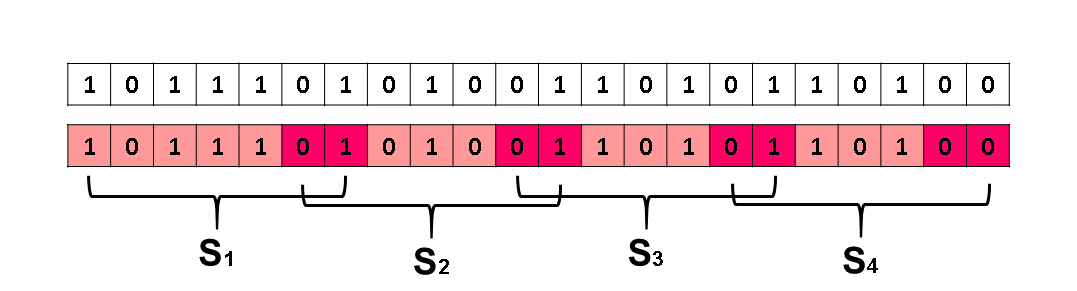
\includegraphics[width=\textwidth]{BDM}
	\caption[Decomposition of a sequence into sub-sequences.]{Decomposition of a sequence of length $|S|=22$ into sub-sequences of length $l=7$ through a sliding window of size $2$, i.e., $m=5$.}
	\label{fig:BDM}
\end{figure}

Thereby, this method combines a local estimation of Kolmogorov complexity with a classical entropy like measure in the long-range \cite{decomposition}.
Finally, it must be mentioned, that in the best case this method approaches better algorithmic complexity than other methods and in the worst case, it behaves just like Shannon-Entropy \cite{decomposition}.

\subsubsection{Generalizations to More Dimensions and Symbols}
If we wish to measure the complexity of sequences of bits in two dimensions, i.e., matrices of $0's$ and $1's$, we can take two approaches. The easiest one is just to flatten the matrix into a unique sequence, this can be achieved by putting each row(or column) of the matrix one in front of the other to form a unique string \cite{kolmo_graph}. 
Another approach is just to generalize our coding theorem and block decomposition methods. Instead of using Turing machines which work out in a 1D tape, we use Turing machines which run over a 2D plane divided into cells \cite{universos}. In this way, the matrices less complex will be those with a greater probability of apparition. For instance, the matrices which are full of zeros or ones must be the less complex. As we can no gather statistics for matrices of all lengths, we can rely again on the block decomposition method to decompose matrices of large dimensions into blocks of matrices of shorter dimensions. An interpretation of this generalized method is that we are seeking the complexity of reconstructing the adjacency matrix associated with a graph from scratch \cite{decomposition}. Thereby, there is an immediate application to graph theory, but also to other objects, such as images, which in the end are matrices. 

Finally, this method can be generalized to any dimensions in the exact same way we discussed for 2-dimensions \cite{decomposition}. Furthermore, the former methods can be generalized to consider Turing machines with more alphabet elements than just $0$ and $1$. For example, with four output symbols, the application could be immediately used to measure the complexity of DNA sequences. Although for the most purposes what we have discussed with two output symbols suffices.


\section{Some Applications of Kolmogorov Complexity}
We end this section commenting on some applications of the K-complexity. We find the main applications in areas where is important to measure the amount of information that an object has because, in the end, this is one of the features that the Kolmogorov complexity allows us to know. Therefore, it has been used in physics, economy, linguistics, psychology, image treatment, image classification, etc \cite{faibles_complexites} \cite{decomposition}. In the area of biology, it could be particularly important in the area of genetics, where researchers are interested in using sequences of DNA data to establish the evolutionary relationship of species \cite{dna}. Among others specific applications we can cite psychometrics \cite{psy}, cellular automata \cite{kolmo_automata1} \cite{kolmo_automata2}, graph theory \cite{kolmo_graph}, machine learning \cite{kolmo_machin1} \cite{kolmo_machin2}, economic time series \cite{kolmo_finan1} \cite{kolmo_finan2}, dynamical systems \cite{kolmo_dynamical}, computer network management \cite{kolmo_computer} and general computation theory \cite{kolmo_computer2}. A compilation of applications to theoretical physics, information and computation can be found in (\cite{kolmo_book}, chapter 8). Finally, in the next chapter, we shall present a novel application of K-complexity to Boolean Networks.